\section{Future Upgrades}
\label{sec:FutureUpgrades}

\subsection{High-Luminosity LHC}
\label{subsec:HLLHC}
The planned High-Luminosity Large Hadron Collider (HL-LHC) is expected to operate starting in mid-2029. The primary goals of the HL-LHC are to collect large quantities of high-quality data needed to study rare SM processes such as Higgs self-interaction, Higgs couplings to lighter particles, the longitudinal component of vector boson scattering processes, and to extend the direct BSM searches beyond the current reach of LHC. The HL-LHC upgrade aims to increase the center-of-mass energy of proton-proton collisions to $\sqrt{s}=14$ TeV and the instantaneous luminosity up to $\mathcal L = 7.5 \times 10^{34} cm^{-2}s^{-1}$ \cite{HLLHC}. Figure \ref{fig:HLLHC} shows the complete operation of LHC starting in 2011 to the planned decade-long HL-LHC program. 

\begin{figure}[!htb]
    \centering
    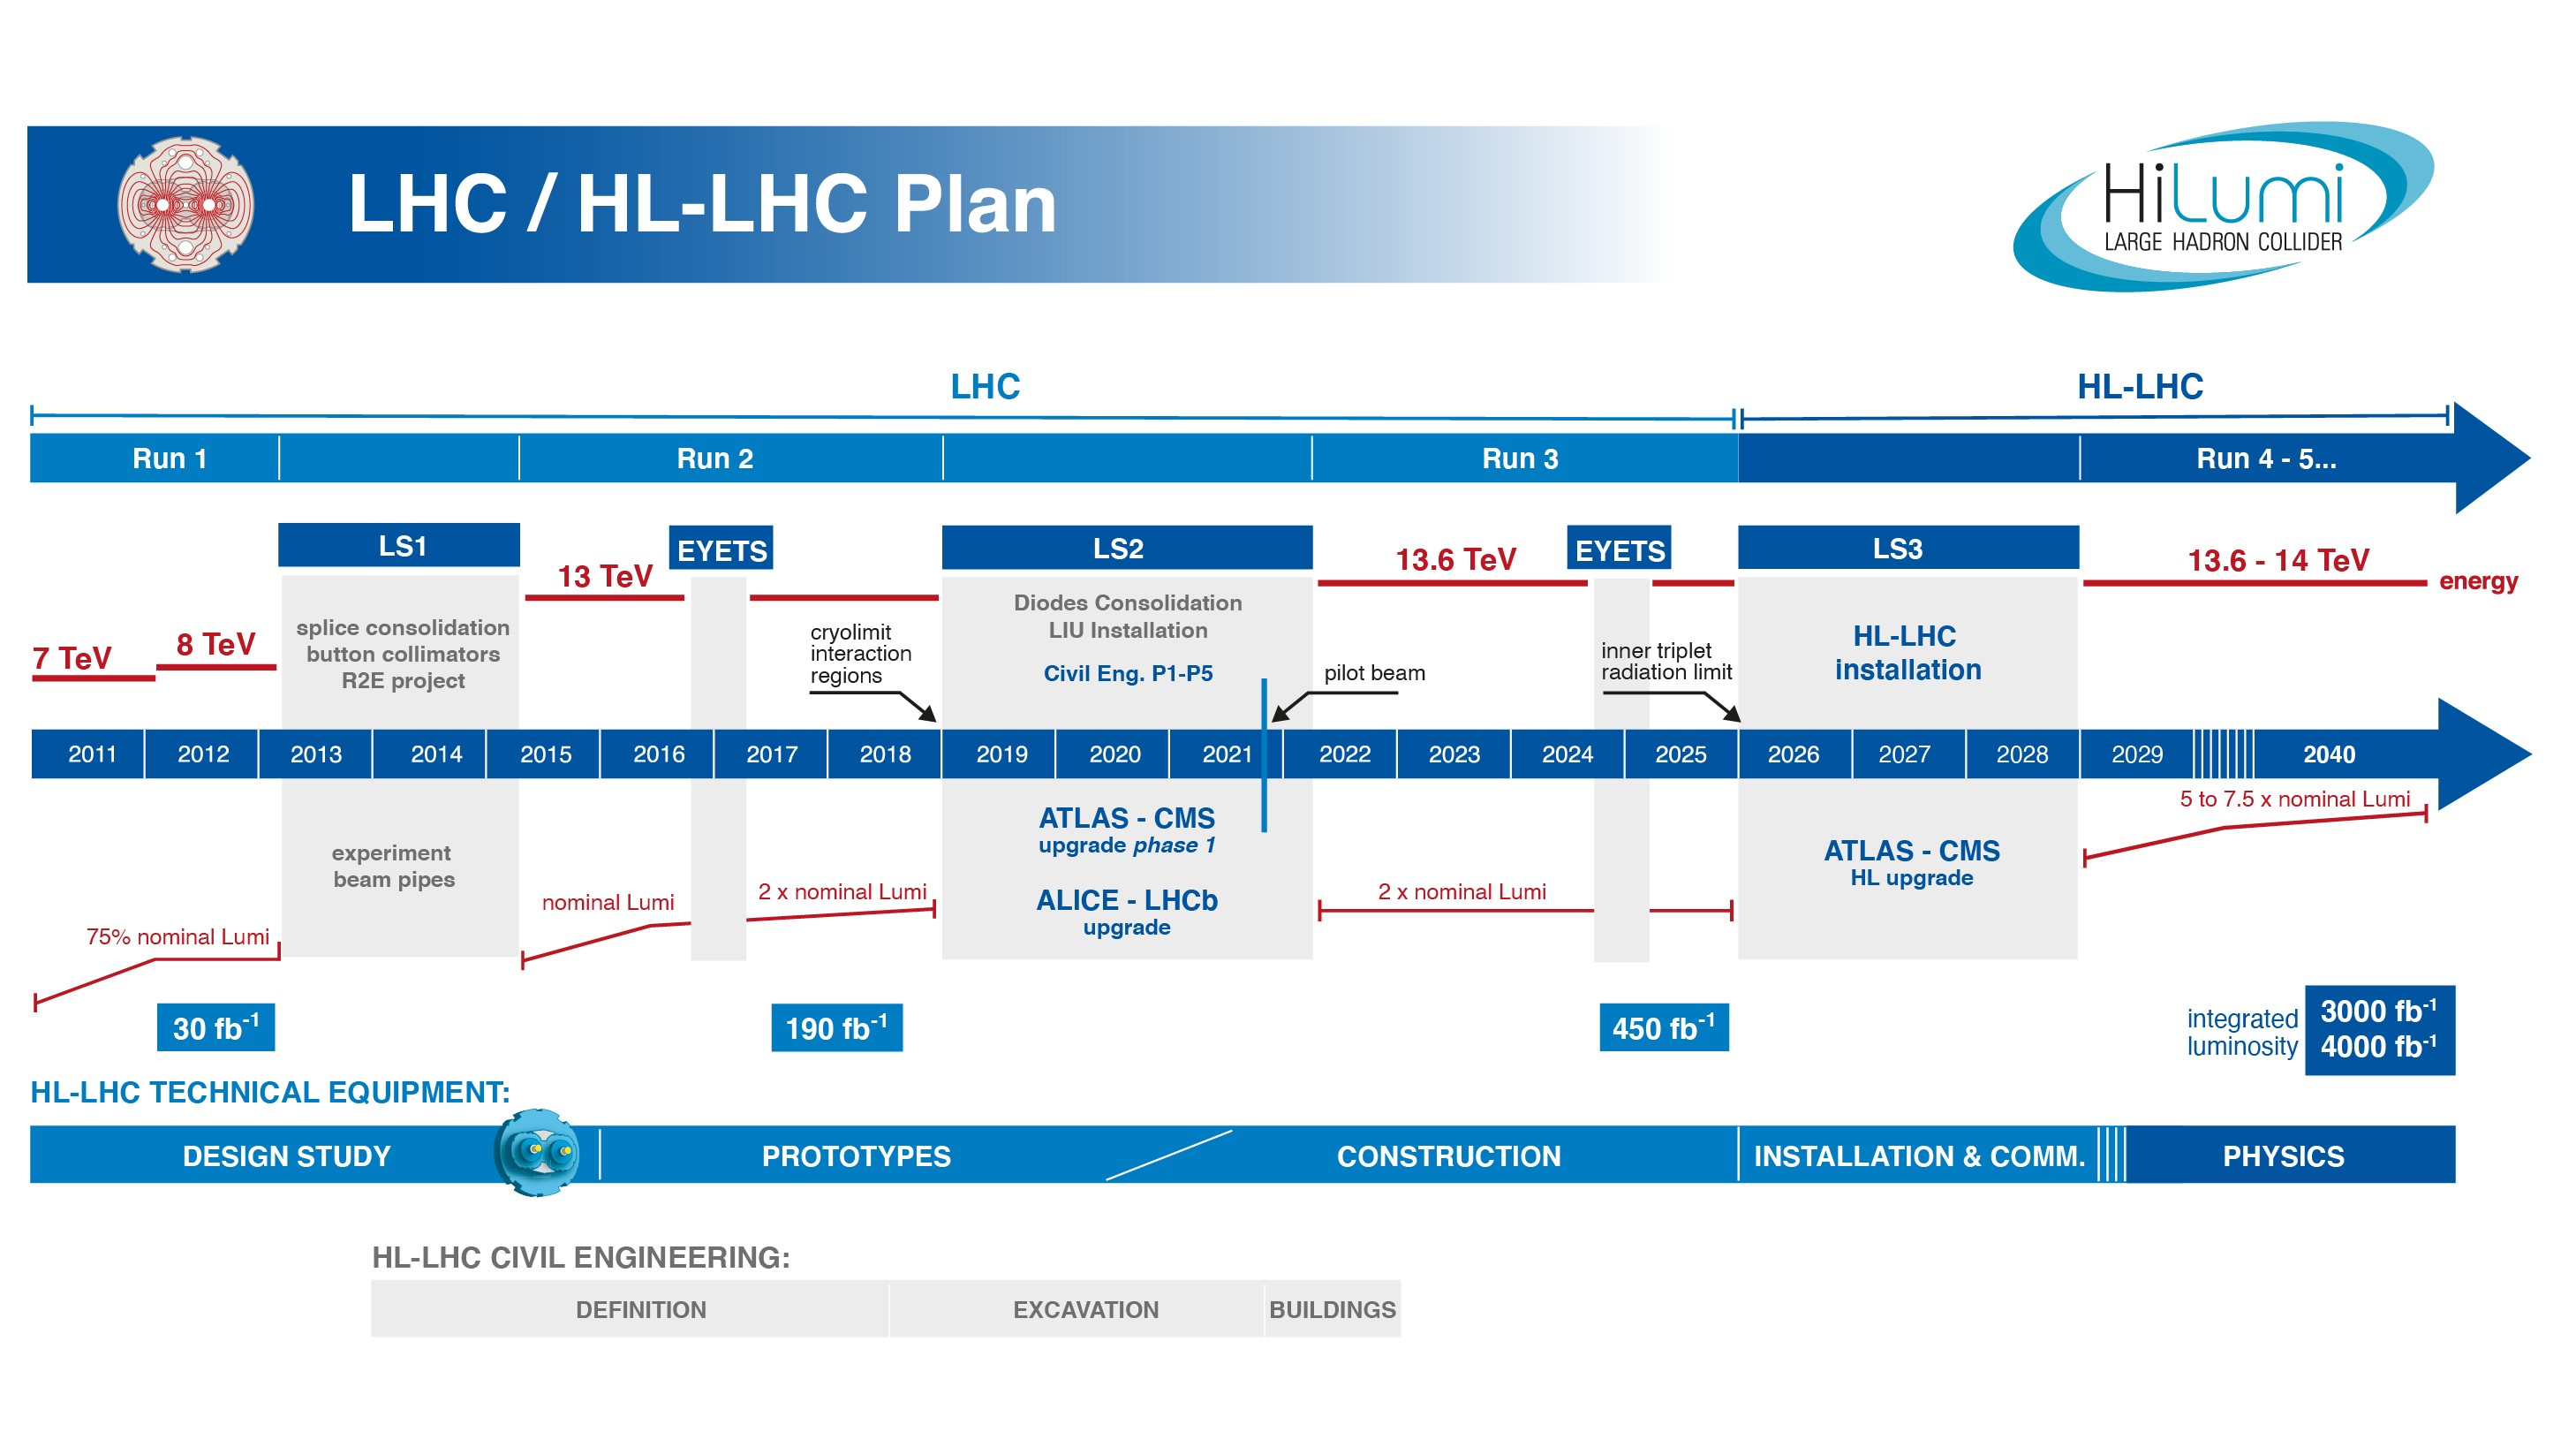
\includegraphics[width=.95\linewidth]{figures/LHC/HLLHCPlan.jpeg}
    \caption{ Timeline of LHC operation starting from 2011 to the planned HL-LHC upgrade. Taken from \small{https://hilumilhc.web.cern.ch/content/hl-lhc-project}.\label{fig:HLLHC}}
\end{figure}
\normalsize

\subsection{ATLAS Upgrades}
\label{subsec:ATLASUpgrade}
The higher center-of-mass energy collisions and about $200$ interactions per bunch crossing at the HL-LHC gives rise to several detector challenges, such as higher detector occupancy, harsher radiation conditions, and higher particle fluxes \cite{HLLHC}. The ATLAS detector will upgrade several sub-systems to meet the challenges of the HL-LHC. The most significant upgrade is replacing the current ID with all-Silicon Inner Tracking (ITk) detector \cite{HLLHC}. Other upgrades include the muon system upgrades, such as the replacement of some MDT chambers in the inner barrel region \cite{HLLHCMuon}, the trigger and data acquisition system upgrade to meet challenges from higher detector occupancy \cite{HLLHCTrigger}, as well as upgrading the electronics of several other sub-systems \cite{HLLHC}. A new High Granularity Timing Detector (HGTD) will also be inserted in the end-cap regions to supplement the tracking system \cite{HLLHC}.

The ITk consists of Silicon pixel and strip detectors to increase granularity and radiation hardness with less material in the detector. Figure \ref{fig:ITKLayout} shows the ITk layout with $5$ inner layers of pixel detector and four outer layers of strips detector. The tracking for ITk is extended in the forward region up to $|\eta| < 4.0$ \cite{ITkStripsTDR}. 

\begin{figure}[!htb]
    \centering
    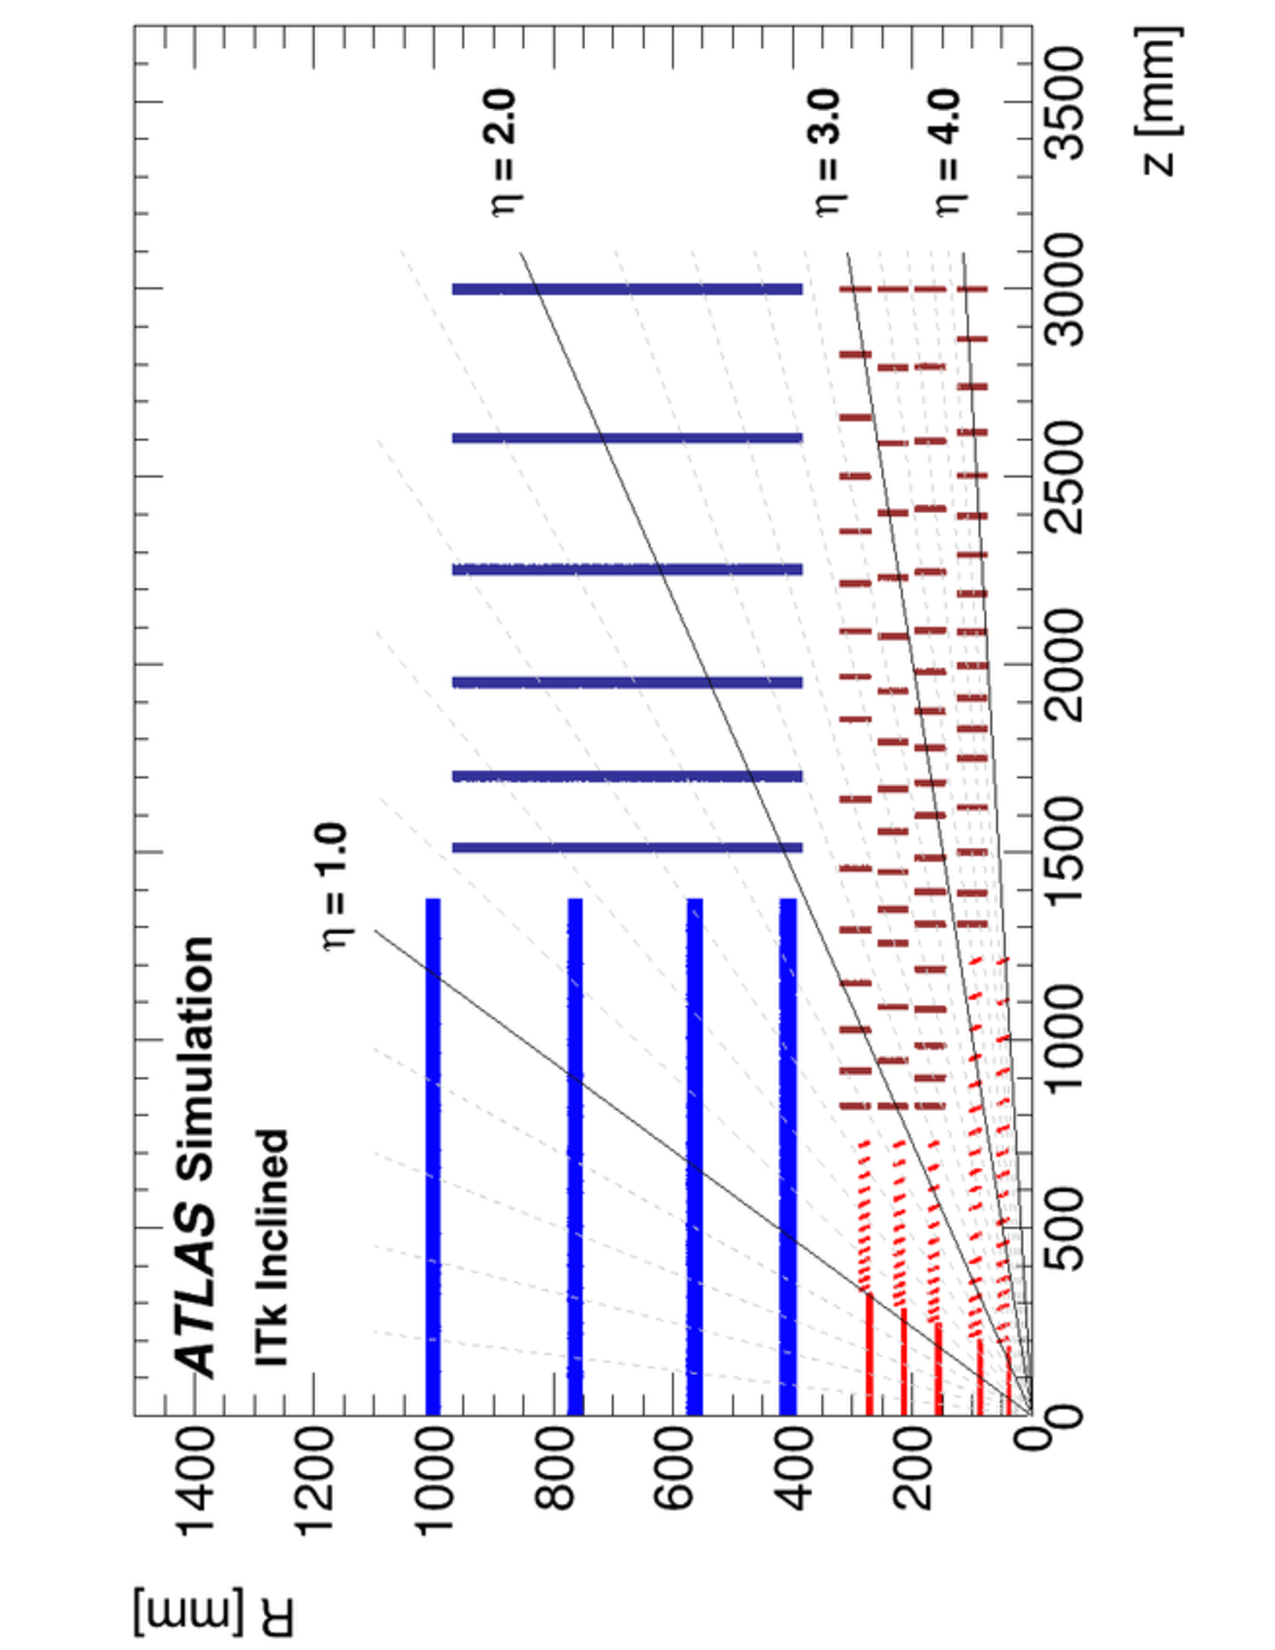
\includegraphics[angle=270,width=.7\linewidth]{figures/LHC/ITKLayout.pdf}
    \caption{ Schematic layout of ITK \cite{ITkPixelTDR}.\label{fig:ITKLayout}}
\end{figure}

At the HL-LHC, the ATLAS experiment is expected to record at least ten times more data than Run-2, making the precision measurements of the rare vector boson scattering process crucial. Identifying and reconstructing the two jets is one of the significant sources of experimental systematic uncertainties in the VBS measurements. Compared to Run-2, at the HL-LHC, the pile-up jet rejection efficiency for the forward jets is expected to increase dramatically due to extended $\eta$ coverage from the ITk \cite{HLLHC_JetTrack}. Moreover, the timing information from the HGTD in the HL-LHC is expected to further improve the forward pile-up jet rejection efficiency up to approximately $30\%$ \cite{HLLHC_HGTD}. Therefore, the HL-LHC program is critical to thoroughly probe the VBS measurements with extremely small cross-sections and two jets in the forward regions.